%-------------------------
% Resume in Latex
% Author : Puneet Gautam, puneet.gautam0206@gmail.com, punitrajgautam@uiit.ac.in
% License : MIT
%MIT License

%Copyright (c) 2023 Puneet Gautam

%Permission is hereby granted, free of charge, to any person obtaining a copy
%of this software and associated documentation files (the "Software"), to deal
%in the Software without restriction, including without limitation the rights
%to use, copy, modify, merge, publish, distribute, sublicense, and/or sell
%copies of the Software, and to permit persons to whom the Software is
%furnished to do so, subject to the following conditions:

%The above copyright notice and this permission notice shall be included in all
%copies or substantial portions of the Software.

%THE SOFTWARE IS PROVIDED "AS IS", WITHOUT WARRANTY OF ANY KIND, EXPRESS OR
%IMPLIED, INCLUDING BUT NOT LIMITED TO THE WARRANTIES OF MERCHANTABILITY,
%FITNESS FOR A PARTICULAR PURPOSE AND NONINFRINGEMENT. IN NO EVENT SHALL THE
%AUTHORS OR COPYRIGHT HOLDERS BE LIABLE FOR ANY CLAIM, DAMAGES OR OTHER
%LIABILITY, WHETHER IN AN ACTION OF CONTRACT, TORT OR OTHERWISE, ARISING FROM,
%OUT OF OR IN CONNECTION WITH THE SOFTWARE OR THE USE OR OTHER DEALINGS IN THE
%SOFTWARE.
%------------------------

%---- Required Packages and Functions ----

\documentclass[a4paper,11pt]{article}
\usepackage{latexsym}
\usepackage{xcolor}
\usepackage{float}
\usepackage{ragged2e}
\usepackage[empty]{fullpage}
\usepackage{wrapfig}
\usepackage{lipsum}
\usepackage{tabularx}
\usepackage{titlesec}
\usepackage{geometry}
\usepackage{marvosym}
\usepackage{verbatim}
\usepackage{enumitem}
\usepackage[hidelinks]{hyperref}
\usepackage{fancyhdr}
\usepackage{multicol}
\usepackage{graphicx}
\usepackage{cfr-lm}
\usepackage[T1]{fontenc}
\setlength{\multicolsep}{0pt} 
\pagestyle{fancy}
\fancyhf{} % clear all header and footer fields
\fancyfoot{}
\renewcommand{\headrulewidth}{0pt}
\renewcommand{\footrulewidth}{0pt}
\geometry{left=0.6cm, top=0.5cm, right=0.6cm, bottom=0.5cm}
% Adjust margins
%\addtolength{\oddsidemargin}{-0.5in}
%\addtolength{\evensidemargin}{-0.5in}
%\addtolength{\textwidth}{1in}
\usepackage[most]{tcolorbox}
\tcbset{
	frame code={}
	center title,
	left=0pt,
	right=0pt,
	top=0pt,
	bottom=0pt,
	colback=gray!20,
	colframe=white,
	width=\dimexpr\textwidth\relax,
	enlarge left by=-2mm,
	boxsep=4pt,
	arc=0pt,outer arc=0pt,
}

\urlstyle{same}

\raggedright
\setlength{\tabcolsep}{0in}

% Sections formatting
\titleformat{\section}{
  \vspace{-4pt}\scshape\raggedright\large
}{}{0em}{}[\color{black}\titlerule \vspace{-7pt}]

%-------------------------
% Custom commands
\newcommand{\resumeItem}[2]{
  \item{
    \textbf{#1}{:\hspace{0.5mm}#2 \vspace{-0.5mm}}
  }
}

\newcommand{\resumePOR}[3]{
\vspace{0.5mm}\item
    \begin{tabular*}{0.97\textwidth}[t]{l@{\extracolsep{\fill}}r}
        \textbf{#1},\hspace{0.3mm}#2 & \textit{\small{#3}} 
    \end{tabular*}
    \vspace{-2mm}
}

\newcommand{\resumeSubheading}[4]{
\vspace{0.5mm}\item
    \begin{tabular*}{0.98\textwidth}[t]{l@{\extracolsep{\fill}}r}
        \textbf{#1} & \textit{\footnotesize{#4}} \\
        \textit{\footnotesize{#3}} &  \footnotesize{#2}\\
    \end{tabular*}
    \vspace{-2.4mm}
}

\newcommand{\resumeProject}[4]{
\vspace{0.5mm}\item
    \begin{tabular*}{0.98\textwidth}[t]{l@{\extracolsep{\fill}}r}
        \textbf{#1} & \textit{\footnotesize{#3}} \\
        \footnotesize{\textit{#2}} & \footnotesize{#4}
    \end{tabular*}
    \vspace{-2.4mm}
}

\newcommand{\resumeSubItem}[2]{\resumeItem{#1}{#2}\vspace{-4pt}}

% \renewcommand{\labelitemii}{$\circ$}
\renewcommand{\labelitemi}{$\vcenter{\hbox{\tiny$\bullet$}}$}

\newcommand{\resumeSubHeadingListStart}{\begin{itemize}[leftmargin=*,labelsep=0mm]}
\newcommand{\resumeHeadingSkillStart}{\begin{itemize}[leftmargin=*,itemsep=1.7mm, rightmargin=2ex]}
\newcommand{\resumeItemListStart}{\begin{justify}\begin{itemize}[leftmargin=3ex, rightmargin=2ex, 
  noitemsep,labelsep=1.2mm,itemsep=0mm]\small}

\newcommand{\resumeSubHeadingListEnd}{\end{itemize}\vspace{2mm}}
\newcommand{\resumeHeadingSkillEnd}{\end{itemize}\vspace{-2mm}}
\newcommand{\resumeItemListEnd}{\end{itemize}\end{justify}\vspace{-2mm}}
\newcommand{\cvsection}[1]{%
\vspace{2mm}
\begin{tcolorbox}
    \textbf{\large #1}
\end{tcolorbox}
    \vspace{-4mm}
}

\newcolumntype{L}{>{\raggedright\arraybackslash}X}%
\newcolumntype{R}{>{\raggedleft\arraybackslash}X}%
\newcolumntype{C}{>{\centering\arraybackslash}X}%
%---- End of Packages and Functions ------




%-------------------------------------------
%%%%%%  CV STARTS HERE  %%%%%%%%%%%
%%%%%% DEFINE ELEMENTS HERE %%%%%%%
\newcommand{\name}{Alessandro Biagiotti} % Your Name
\newcommand{\course}{Magistrale in Informatica} % Your Course
%\newcommand{\roll}{Your Roll No} % Your Roll No.
\newcommand{\phone}{3917572924} % Your Phone Number
\newcommand{\email}{alexbgtt@gmail.com} %Email 
\newcommand{\github}{S3gmentati0nFault} %Github
\newcommand{\website}{https://www.aboringsite.com/} %Website
\newcommand{\linkedin}{alessandro-biagiotti-a863a81a2/} %linkedin




\begin{document}
\fontfamily{cmr}\selectfont
%----------HEADING-----------------
\parbox{5.25cm}{%

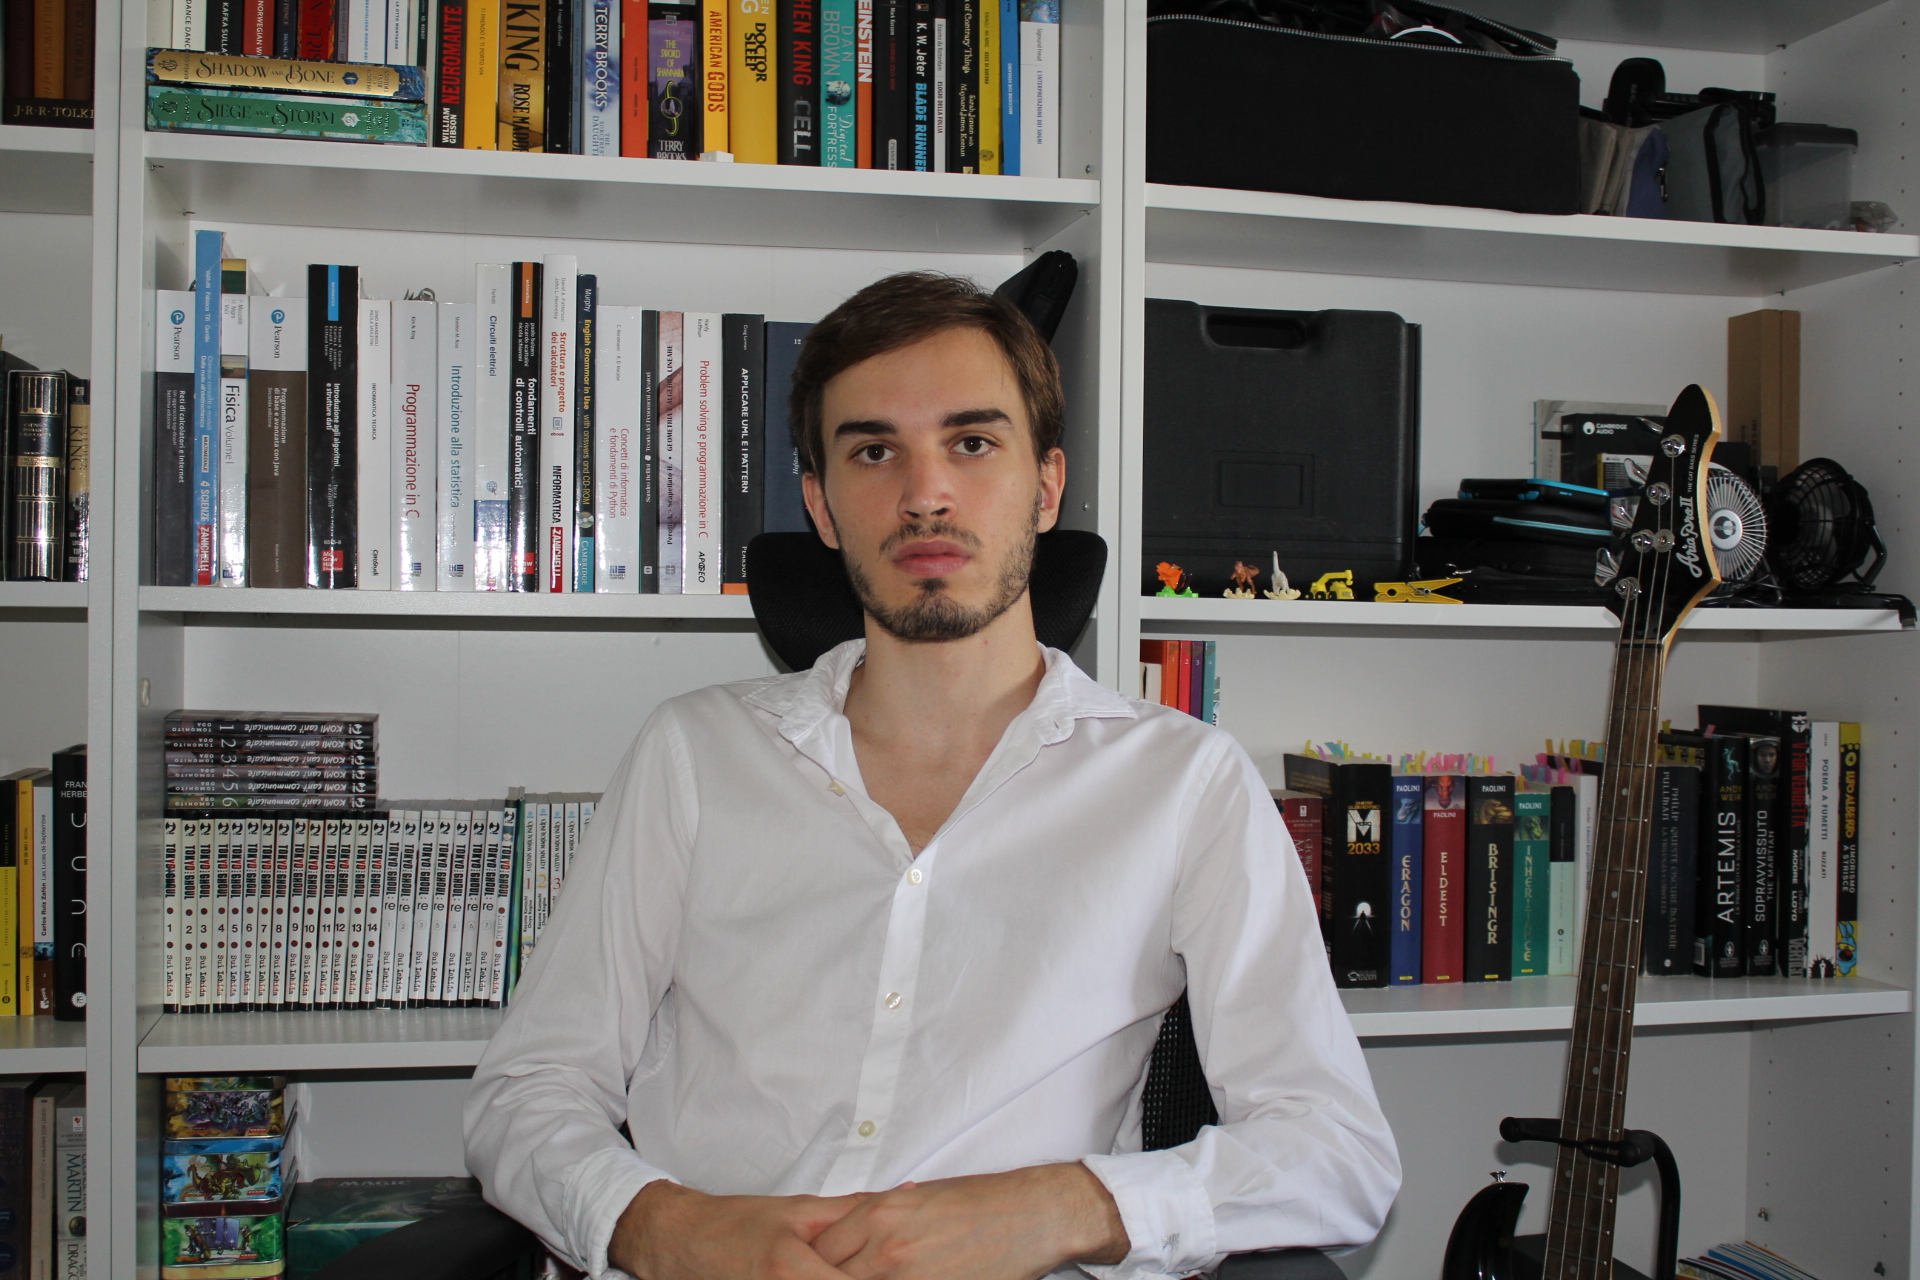
\includegraphics[width=5cm,clip]{foto_curriculum.JPG}

}\parbox{\dimexpr\linewidth-5.25cm\relax}{
\begin{tabularx}{\linewidth}{L r}
  \textbf{\LARGE \name} & +39-\phone\\
  
  \course &  \href{mailto:\email}{\email}\\
   &  \href{https://github.com/\github}{GitHub} \\
   &  \href{\website}{A Boring Site}\\
  {Universitá degli studi di Milano, Milano} & \href{https://www.linkedin.com/in/\linkedin/}
  {LinkedIn}
\end{tabularx}
}

\vspace{-0.5mm}
%-------------SUMMARY-----------------
\section{\textbf{Presentazione}}
Sono abituato a lavorare piú degli altri perché devo compensare il fatto che mi é necessario piú tempo per 
imparare le corse.\\
Ho molti interessi e cerco di tenerli sempre vivi nonostante gli impegni durante la settimana la rendano 
un'impresa difficile.\\
Mi fa sempre molto piacere essere a contatto con altre persone perché sento il bisogno di essere sempre la 
mia miglior versione. Mi piace imparare dagli altri e che gli altri imparino da me in una condizione di 
libero aiuto reciproco.\\
Qual'é il mio piú grande punto di forza? Riesco ad adattarmi facilmente alle situazioni e a inserirmi nei 
contesti giá avviati o in corso di avviamento.\\
Qual'é la mia piú grande debolezza? Mi scoraggio troppo facilmente.

%-----------EDUCATION-----------------
\section{\textbf{Curriculum universitario}}
\setlength{\tabcolsep}{5pt} % Default value: 6pt
% \renewcommand{\arraystretch}{1.1} % Default value: 1
\small{\begin{tabularx}
{\dimexpr\textwidth-2mm\relax}{|c|C|c|c|}
  \hline
  \textbf{Degree } & \textbf{Institute} & \textbf{Average} & 
  \textbf{Year}\\
  \hline
  Magistrale & Universitá degli studi di Milano & 28 (Fino al primo semestre) & 
  Odierno\\
 
  \hline
  Triennale & Universitá degli studi di Milano Bicocca & 26 & 2020 - 2022 \\
  \hline
  Triennale & Politecnico di Milano & 23 & 2018-2020 \\
  \hline
\end{tabularx}}
\vspace{-1mm}

%-----------EXPERIENCE-----------------
\section{\textbf{Esperienze pregresse}}
  \resumeSubHeadingListStart

    \resumeSubheading
      {Certimeter Srl}{Torino}
      {Tirocinante}{Febbraio 2022 - Luglio 2022}
      \resumeItemListStart
        \item {L'obiettivo del tirocinio era quello di creare un'applicazione web 
        distribuita utilizzando tecnologie come Docker, Spring Framework e React JS
        }
      \resumeItemListEnd

    \resumeSubheading
      {Comune di Milano}{Milano}
      {Scrutatore}{}
      \resumeItemListStart
        \item \textit{Ottobre 2021} - Elezioni amministrative
        \item \textit{Settembre 2022} - Elezioni Politiche
        \item \textit{Febbraio 2023} - Elezioni Regionali
      \resumeItemListEnd
    
%    \vspace{-1mm}
%    \resumeSubheading
%      {Company Name}{Location}
%      {Position}{June 2021 - July 2021}
%      \resumeItemListStart
%    \item {About work}
%    \item {About Work}
%    \resumeItemListEnd
    
    
    % \item {More work done } .....

    
  
      
  \resumeSubHeadingListEnd
\vspace{-6.5mm}
%-----------PROJECTS-----------------
\section{\textbf{Progetti}}
\resumeSubHeadingListStart
    \resumeProject
      {Pump Down The Flame} %Project Name
      {corso Game Design and Programming} %Project Name, Location Name
      {Nov 2022 - Feb 2023} %Event Dates
      {
        \href{https://polimi-game-collective.itch.io/pump-down-the-flame/devlog/486076/update-beta-version-v110}
        {\textbf{Itch.io}}
      } %Website
      \resumeItemListStart
        \item {Design e implementazione del gioco originale "Pump Down The Flame"}
        \item {Probabilmente il gioco riceverá altri aggioernamenti per Giugno 2023 quando
        verrá hostato il Game Jam del Politecnico di Milano}
      \resumeItemListEnd

    \resumeProject
      {Anagrafica Aziendale} %Project Name
      {Progetto di Tirocinio} %Project Name, Location Name
      {Feb 2022 - Lug 2022} %Event Dates
      {\href{https://github.com/Andrea-Perego-99/Anagrafica-Aziendale}{\textbf{Github}}} %Website
      \resumeItemListStart
        \item {Applicazione distribuita che gestisce i dati degli impiegati in sicurezza}
      \resumeItemListEnd
    
     \vspace{-1mm}
     
    \resumeProject
      {Notepad} %Project Name
      {corso Programmazione in C++} %Project Name, Location Name
      {Dic 2021 - Gen 2022} %Event Dates
      {
        %\href{Github Link}{\textbf{Github}}
      } %Website
      \resumeItemListStart
        \item {Piccola applicazione in QT che puó essere utilizzata come blocco note}
        \item {Era necessario che consentisse le seguenti operazioni:
          \begin{itemize}
            \item Salvare e aprire un file
            \item Cercare parole o frasi all'interno del file
          \end{itemize}
        }
      \resumeItemListEnd

    \resumeProject
      {Sparse Matrix} %Project Name
      {corso Programmazione in C++} %Project Name, Location Name
      {Dic 2021 - Gen 2022} %Event Dates
      {
        %\href{Github Link}{\textbf{Github}}
      } %Website
      \resumeItemListStart
        \item {Implementazione di una soluzione che consentisse di mantenere in memoria 
        matrici sparse impiegando la minima quantitá di memoria possibile}
      \resumeItemListEnd

    \resumeProject
      {Algoritmo di Prim} %Project Name
      {corso Linguaggi di programmazione} %Project Name, Location Name
      {Nov 2020 - Gen 2021} %Event Dates
      {
        %\href{Github Link}{\textbf{Github}}
      } %Website
      \resumeItemListStart
        \item { Implementazione dell'algoritmo di Prim utilizzando i linguaggi Prolog e Common-lisp 
        rimanendo al di sotto di una determinata soglia di risorse utilizzate}
      \resumeItemListEnd

    \resumeProject
      {Implementazione di un RB tree} %Project Name
      {corso Algoritmi e Strutture dati} %Project Name, Location Name
      {Jun 2019 - Sett 2019} %Event Dates
      {
        %\href{Github Link}{\textbf{Github}}
      } %Website
      \resumeItemListStart
        \item {Implementazione della struttura impiegando la minor quantitá di memoria possibile}
      \resumeItemListEnd
      
\resumeSubHeadingListEnd
\vspace{-7.5mm}

\section{\textbf{Technical Skills}}
 \resumeHeadingSkillStart
  \resumeSubItem{Linguaggi di programmazione in ordine di esperienza} % Category
    { C++, HTML, CSS, JavaScript, Java, C\#, C, Common-Lisp, Prolog, Python}
    
    %\vspace{-0.5mm}
    
 \resumeSubItem{Tools and Frameworks} % Category
    {Visual Studio, CLion, Intellij Idea, Intellij Rider, React JS, Docker} % Skills
    
    %\vspace{-0.5mm}
    
 \resumeSubItem{Operating Systems} % Category
    {Windows, Linux, Mac OS} % Skills
    
    %\vspace{-0.5mm}
    
 
 \resumeHeadingSkillEnd

\vspace{-1.5mm}

\section{\textbf{Alcuni corsi sostenuti}}
\resumeHeadingSkillStart
 \resumeSubItem{Corsi di informatica} % Category
    {C Programming, Object Oriented Programming 1 \& 2, Database, Programming Languages, 
    C++ Programming, Videogame Design and Programming, Software Engineering, 
    Computer Architectures \& Operating Systems, Computer Networks, Distributed Systems, 
    Algorithms and data structures}
    %\vspace{-0.5mm}
 \resumeSubItem{Altri corsi}
 {Calculus 1 \& 2, Physics \& Thermodynamics, Geometry and applied Algebrae, Automation, Ricerca operativa}
%  \resumeSubItem{Electrical and Electronics} % Category
%     {Advanced Control Systems, Digital Systems, Microprocessors} % Skills
\resumeHeadingSkillEnd

\vspace{-1mm}
%---------------CERTIFICATIONS-------------------
\section{\textbf{Certificazioni}}
    \resumeItemListStart
        \item {\textbf{ Versant English placement test}}
        {Universitá degli studi di Milano - C1 english certification}%Certifying Authority
        \item {\textbf{ First For English}}
        {Cambridge English - B2.2 english certification} %Certifying Authority
    \resumeItemListEnd
\vspace{-4mm}

%-----------TRAINING-----------------
% \section{\textbf{Vocational Training}}
%   \resumeSubHeadingListStart
%     \resumeSubheading
%       {Institution Name}{Location}
%       {Course Name}{Start Time-EndTime}
%       \resumeItemListStart
%         \item {About course, blah blah}
%         \item {About course, blah blah}
%       \resumeItemListEnd 
%     \resumeSubHeadingListEnd


% \section{\textbf{Positions of Responsibility}}
% \vspace{-0.4mm}
% \resumeSubHeadingListStart
%   \resumePOR{Secretary} % Position
%     {XYZ Club, UIT Shimla} %Club,Event
%     {Apr. 2018 - Apr. 2019} %Tenure Period
%   \resumePOR{Secretary} % Position
%     {XYZ Club, UIT Shimla} %Club,Event
%     {Apr. 2018 - Apr. 2019} %Tenure Period
% \resumeSubHeadingListEnd
% \vspace{-4mm}


\section{\textbf{Progetti personali}}
\vspace{-0.1mm}
\resumeSubHeadingListStart
\resumeProject
  {\href{https://www.aboringsite.com/}{\textbf{A Boring Site}}} %Project Name
  {Sito di informazione} %Project Name, Location Name
  {2021 - Odierno} %Event Dates
  {
  %\href{Github Link}{\textbf{Github}}
  } %Website
  \resumeItemListStart
  \item {Sito nato dalla collaborazione con un amico, l'obiettivo é quello di fare informazione riguardo a 
  temi non banali con rigore.}
  \resumeItemListEnd

\resumeProject
  {\href{https://open.spotify.com/show/5mKtG1VeiAUcUcDIqKHrYL?si=a00a07d9f7574171}
  {\textbf{A Boring Podcast}}} %Project Name
  {Cultural podcast} %Project Name, Location Name
  {2021 - Current} %Event Dates
  {
  %\href{Github Link}{\textbf{Github}}
  } %Website
  \resumeItemListStart
  \item {Il podcast é nato dalla collaborazione con un amico nel tentativo di spiegare ai piú argomenti 
  complessi con l'aiuto di persone del settore.}
  \resumeItemListEnd

% \resumePOR{Achievement 1} % Award
%     {About it} % Event
%     {2021} %Event Year
% \vspace{-0.1mm}
% \resumePOR{Achievement 2} % Award
%     {About it} % Event
%     {2021} %Event Year
% \vspace{-0.1mm}
\resumeSubHeadingListEnd
%-------------------------------------------
\vfill
%\center{\footnotesize Last updated: \today}

\end{document}
